\documentclass[conference]{IEEEtran}
% \IEEEoverridecommandlockouts
% The preceding line is only needed to identify funding in the first footnote. If that is unneeded, please comment it out.
%Template version as of 6/27/2024

\usepackage{cite}
\usepackage{amsmath,amssymb,amsfonts}
\usepackage{algorithmic}
\usepackage{graphicx}
\usepackage{textcomp}
\usepackage{xcolor}
\usepackage{amsthm}
\usepackage{algorithm}
\newtheorem{definition}{Definition}
\def\BibTeX{{\rm B\kern-.05em{\sc i\kern-.025em b}\kern-.08em
    T\kern-.1667em\lower.7ex\hbox{E}\kern-.125emX}}
\begin{document}

\title{Impact of Parameters on\\ Random Forests}

\author{\IEEEauthorblockN{Tasheel Govender}
\IEEEauthorblockA{\textit{Principles of Data Science - 771} \\
\textit{Stellenbosch University}\\
25002112@sun.ac.za}}

\maketitle

\begin{abstract}
This study presents a systematic investigation into the effects of key parameters on the performance of random forests for classification tasks. Using three benchmark datasets of varying complexity including wine, adult income, and MNIST, the study explores the impact and relationship between parameters and how they influence model accuracy, confidence, and diversity. Additionally, the report examines the impact of constructing heterogeneous ensembles with diverse tree configurations. Experimental results, obtained through rigorous cross-validation and multiple evaluation metrics, reveal that optimal parameter settings depend on dataset characteristics and complexity. The findings provide practical insights for model selection and parameter tuning, emphasizing the importance of ensemble diversity and careful configuration in achieving robust predictive performance.
\end{abstract}

\section{Introduction}

Machine learning has become an essential tool for extracting patterns and making predictions from complex datasets. Among the various approaches, ensemble methods have gained prominence due to their ability to combine multiple models to achieve improved predictive performance and robustness. Random forests, a widely used ensemble technique, leverage the strengths of decision trees while mitigating their limitations through randomization and aggregation.

This report investigates the influence of key parameters on the performance of random forests across datasets of varying complexity. The analysis encompasses a systematic exploration of tree depth, the number of features considered at each split and the relationship between tree depth and the number of trees in the ensemble. In addition, the study evaluates the impact of constructing heterogeneous ensembles, where individual trees are assigned diverse parameter configurations. The empirical procedure includes rigorous cross-validation and the use of multiple evaluation metrics to ensure reliable and comprehensive assessment.

The results presented in this report provide insights into how parameter choices affect model accuracy, confidence, and diversity. The findings highlight the interplay between dataset characteristics and optimal random forest configurations. The report concludes with a discussion of the implications for model selection and parameter tuning in practical applications.

\section{Background}

Ensemble learning refers to the process of generating and combining multiple inducers, where an inducer is a machine learning algorithm or model trained to solve a specific predictive task such as classification or regression~\cite{https://doi.org/10.1002/widm.1249}. The central concept of ensemble learning is that aggregating the predictions of multiple models yields higher accuracy than relying on a single model.

\subsection{Bootstrap Aggregating}

Several methods exist for creating ensembles. One widely used approach is bootstrap aggregating, also known as bagging~\cite{Breiman1996}. Bagging generates an ensemble of independent models, with each inducer trained on a bootstrap sample drawn with replacement from the original dataset. Typically, each bootstrap sample contains the same number of instances as the original dataset, ensuring that each inducer is trained on a sufficiently large set of data~\cite{https://doi.org/10.1002/widm.1249}. Bagging is formally defined as follows~\cite{Buhlmann2002}:

\begin{definition}[Bagging]
\begin{enumerate}
    \item Construct a bootstrap sample $L^*_i = (Y^*_i, X^*_i)$ for $i = 1, \ldots, n$ according to the empirical distribution of the pairs $L_i = (Y_i, X_i)$ for $i = 1, \ldots, n$.
    \item Compute the bootstrapped predictor $\hat{\theta}^*_n(x)$ by the plug-in principle, that is,
    \[
        \hat{\theta}^*_n(x) = h_n(L^*_1, \ldots, L^*_n)(x),
    \]
    where $\hat{\theta}_n(x) = h_n(L_1, \ldots, L_n)(x)$.
    \item The bagged predictor is
    \[
        \hat{\hat{\theta}}_{n;B}(x) = \mathbb{E}^*\left[\hat{\theta}^*_n(x)\right].
    \]
\end{enumerate}
\end{definition}

This definition describes the process of bagging. Multiple new datasets are created by randomly sampling from the original data with replacement. A separate model is trained on each bootstrap sample. The final prediction is obtained by aggregating the outputs of all models, which improves accuracy and stability compared to using a single model.

\subsection{Random Forests}

A special case of bagging that utilizes decision trees as base learners is the random forest. Random forests construct multiple decision trees and combine the predictions by majority vote for classification or by averaging for regression tasks~\cite{10.1007/978-3-642-31537-4_13}. Random forests were formally introduced in 2001 by Leo Breiman~\cite{Breiman2001}. The development of random forests was influenced by earlier work by Amit and Geman~\cite{10.1162/neco.1997.9.7.1545} on shape recognition using randomized decision trees, and by Ho~\cite{Ho1995} on random decision forests. Breiman showed, using the law of large numbers, that the generalization error of a random forest converges to a limit as the number of trees in the forest increases. This result indicates that adding more trees to the ensemble does not lead to overfitting, making random forests a robust and reliable method for various machine learning tasks.

\begin{algorithm}[H]
    \caption{Random Forest Algorithm}
    \label{alg:random_forest}
\begin{algorithmic}[1]
\REQUIRE Training set $D = \{(x_1, y_1), \ldots, (x_n, y_n)\}$, number of trees $T$, number of features $m$
\ENSURE Random forest model $F$
\FOR{$t = 1$ to $T$}
    \STATE Draw a bootstrap sample $D_t$ from $D$
    \STATE Train a decision tree $h_t$ on $D_t$:
        \FOR{each node in $h_t$}
            \STATE Randomly select $m$ features from all features
            \STATE Find the best split among the $m$ features
        \ENDFOR
\ENDFOR
\STATE \textbf{Output:} $F = \{h_1, h_2, \ldots, h_T\}$
\STATE For prediction on new instance $x$:
    \STATE \hspace{1em} For classification: return the majority vote $\text{mode}(h_1(x), \ldots, h_T(x))$
    \STATE \hspace{1em} For regression: return the average $\frac{1}{T} \sum_{t=1}^T h_t(x)$
\end{algorithmic}
\end{algorithm}

Algorithm~\ref{alg:random_forest} outlines the steps involved in constructing a random forest. Each tree is built using a bootstrap sample of the data, and at each node, a random subset of features is considered for splitting. The final prediction is made by aggregating the outputs of all trees in the forest.

\subsection{Random Feature Selection}

Random feature selection is a key component of the random forest algorithm that enhances model diversity and reduces overfitting. Ho~\cite{Ho1995} introduced the concept of random feature selection in random decision forests. In this approach, at each split in a decision tree, a random subset of features is selected from the total set of features. The best feature for splitting is then chosen from this subset rather than from the entire feature set.

Ho demonstrated that this randomization technique leads to a significant reduction in correlation among the individual trees in the ensemble, which in turn improves the overall performance of the random forest. By limiting the feature set considered at each split, random feature selection helps to create more diverse trees, which is crucial for the success of ensemble methods such as random forests.

\subsection{Limitations}

Despite their popularity and strong predictive performance, random forests have several limitations. One major drawback is the bias towards features with many categories, which may lead to misleading variable importance measures~\cite{Louppe2014}. Additionally, training and prediction can be computationally intensive for large datasets, as the method requires constructing and evaluating many trees. These limitations highlight the importance of careful parameter tuning and consideration of alternative methods when interpretability or computational efficiency is critical.

\section{Implementation}

The random forest algorithm was implemented using Python in a Jupyter Notebook environment. The primary libraries used included Scikit-learn for machine learning functionalities, Pandas for data manipulation, and NumPy for numerical computations. Matplotlib and Seaborn were used for data visualization. This section describes the data processing steps, the random forest algorithm, and the experimental setup used to evaluate model performance. The source code for the implementation is available on Github\footnote{https://github.com/TasheelGovender/ML\_assignment\_4}.

\subsection{Data}

The datasets chosen for this study are the wine dataset~\cite{Lichman2013wine}, the adult income dataset~\cite{Dheeru2017adult}, and the MNIST dataset~\cite{LeCun1998mnist}. These datasets were sourced from the UCI Machine Learning Repository~\cite{Dua2019} and are commonly used for benchmarking machine learning algorithms. Table~\ref{tab:dataset_summary} provides a summary of the datasets used in this study, including the number of instances, features, and their complexity levels.

\begin{table}[htbp]
    \caption{Dataset Summary}
    \label{tab:dataset_summary}
    \centering
    \begin{tabular}{|l|c|c|c|}
        \hline
        \textbf{Dataset} & \textbf{Instances} & \textbf{Features} & \textbf{Complexity} \\
        \hline
        Wine & 178 & 13 & Low \\
        Adult & 48,842 & 14 & Medium \\
        MNIST & 70,000 & 784 & High \\
        \hline
    \end{tabular}
\end{table}

To prepare the data for the random forest algorithm, several preprocessing steps were undertaken. Instances with missing values were removed. The target variables were identified and encoded for classification tasks. The adult income and MNIST datasets were sampled to reduce computational load during experimentation. Stratified sampling was used to create a sample of 10,000 instances from each dataset to maintain the class distribution.

\subsection{Experimentation}

The experimentation involved four separate experiments to evaluate the impact of various parameters and the performance of different random forest configurations. The experiments conducted are as follows:

\subsubsection{Experiment 1}

This experiment explores the impact of varying tree depths. A random forest model was trained with different maximum tree depths to observe how this parameter affects model performance and overfitting. Scikit-learn's \texttt{RandomForestClassifier} was used for the model implementation. A range of maximum tree depths from 1 to 30, as well as no maximum depth, was evaluated. All other parameters were kept constant, including the number of trees and the number of features considered at each split. The \texttt{class\_weight} parameter for the \texttt{RandomForestClassifier} was set to \texttt{balanced} to address any class imbalance in the datasets. Cross-validation with 8 folds was employed using the \texttt{StratifiedKFold} class from Scikit-learn to ensure robust evaluation of model performance across different tree depths.

\subsubsection{Experiment 2}

This experiment evaluates the relationship between the number of trees and the tree depth. The \texttt{RandomForestClassifier} was used to train models with a varying number of trees and maximum tree depths. The number of trees was increased incrementally from 10 to 300, while the maximum depth was varied from 1 to 30, as well as no maximum depth. The number of features considered at each split was kept constant for this experiment. A \texttt{balanced} class weight was used to address any class imbalance in the datasets. Cross-validation with 8 folds was again employed using the \texttt{StratifiedKFold} class from Scikit-learn to ensure robust evaluation of model performance across different configurations of tree numbers and depths.

\subsubsection{Experiment 3}

This experiment explores the impact of the number of randomly selected features at each split. As in Experiment 1, the \texttt{RandomForestClassifier} was used to train models. In this experiment, the number of features considered at each split was varied. The values ranged from 1 to 100, as well as the square root and logarithm (base 2) of the total number of features. Fractions of the total number of features were also used, specifically 25\% and 50\%. The number of trees and maximum tree depth were kept constant using the best parameters found in Experiment 1. A \texttt{balanced} class weight was used to address any class imbalance in the datasets. Cross-validation with 8 folds was again employed using the \texttt{StratifiedKFold} class.

\subsubsection{Experiment 4}

This experiment explores the performance of a heterogeneous ensemble of decision trees with varying parameters. A custom implementation was developed to construct an ensemble in which each decision tree is assigned a unique combination of maximum tree depth and number of features considered at each split.

Algorithm~\ref{alg:heterogeneous_ensemble} outlines the steps involved in constructing a heterogeneous ensemble of decision trees with varying parameters. Cross-validation was again used to evaluate the performance of this ensemble approach.

\begin{algorithm}[H]
\caption{Heterogeneous Ensemble with Bagging and Parameter Variation}
\label{alg:heterogeneous_ensemble}
\begin{algorithmic}[1]
\REQUIRE Training data $(X, y)$, list of tree depths $\mathcal{D}$, list of max\_features values $\mathcal{F}$, number of trees $N$
\ENSURE Ensemble of decision trees with diverse parameters

\STATE Generate all possible $(\text{depth}, \text{max\_features})$ pairs: $\mathcal{P} = \mathcal{D} \times \mathcal{F}$
\STATE Assign a $(\text{depth}, \text{max\_features})$ pair to each tree: for $i = 1$ to $N$, set $\text{params}_i = \mathcal{P}[i \bmod |\mathcal{P}|]$
\FOR{$i = 1$ to $N$}
    \STATE Draw a bootstrap sample $(X_i, y_i)$ from $(X, y)$ (sampling with replacement)
    \STATE Train decision tree $T_i$ with $\text{params}_i$ on $(X_i, y_i)$
\ENDFOR
\STATE \textbf{Prediction:}
\FOR{each test instance $x$}
    \FOR{$i = 1$ to $N$}
        \STATE Obtain predicted class probabilities $p_i = T_i.\text{predict\_proba}(x)$
    \ENDFOR
    \STATE Compute average probability: $\bar{p} = \frac{1}{N} \sum_{i=1}^N p_i$
    \STATE Assign final class label as $\arg\max_j \bar{p}_j$
\ENDFOR
\end{algorithmic}
\end{algorithm}


\section{Empirical Procedure}

\subsection{Control Parameters}

For \textit{Experiment 1}, the ensemble consisted of 100 trees, and the number of features considered at each split was set to the square root of the total number of features. This configuration typically provides a sufficient number of estimators to achieve stable and reliable predictions while avoiding unnecessary computational overhead. The square root heuristic effectively balances randomness and informativeness, promoting diversity among trees and reducing the risk of overfitting.

\textit{Experiment 2} used the best maximum tree depth found in \textit{Experiment 1}, and the number of features considered at each split was again set to the square root of the total number of features.

\textit{Experiment 3} used the best parameters identified in the previous experiments for the number of trees and maximum tree depth.

Finally, \textit{Experiment 4} tested a heterogeneous ensemble of decision trees with varying parameters, where each tree was assigned a unique combination of parameters.

\subsection{Evaluation Metrics}

To evaluate the performance of the random forest models across the different experiments, several evaluation metrics were employed. These metrics were chosen to provide a comprehensive assessment of model performance, particularly in the context of classification tasks. Cross-validation with 8 folds was used to ensure robust evaluation and to mitigate the effects of overfitting.

The metrics for all experiments include accuracy, F1 score, recall, standard deviation of predicted probabilities, and confusion matrices. Accuracy measures the proportion of correct predictions, while F1 score balances precision and recall, making it suitable for datasets with class imbalance. Recall quantifies the model's ability to identify positive instances. The standard deviation of predicted probabilities provides insight into the confidence of the model's predictions. Confusion matrices were generated to visualize model performance across different classes, allowing for detailed analysis of true positives, false positives, true negatives, and false negatives.

For \textit{Experiment 4}, in addition to the metrics mentioned above, precision and diversity measures were also calculated. Precision assesses the accuracy of positive predictions, which is important in scenarios where false positives carry significant consequences. Diversity measures were computed to evaluate the heterogeneity of the ensemble, as increased diversity among models can improve overall performance by reducing correlation among individual trees.
\section{Research Results}

Figure~\ref{fig:accuracy_vs_depth} shows the accuracy results from \textit{Experiment 1}, where the impact of varying tree depths on model performance was evaluated. For the wine dataset, the accuracy starts off high at a depth of 1 and increases slightly as the depth increases, reaching a peak at depth 3 before stabilizing. This result is expected because the wine dataset is relatively simple and does not require deep trees to capture the underlying patterns. For simple datasets, shallow trees are often sufficient to achieve good performance, and increasing the depth may not provide significant benefits.


\begin{figure}
    \centering
    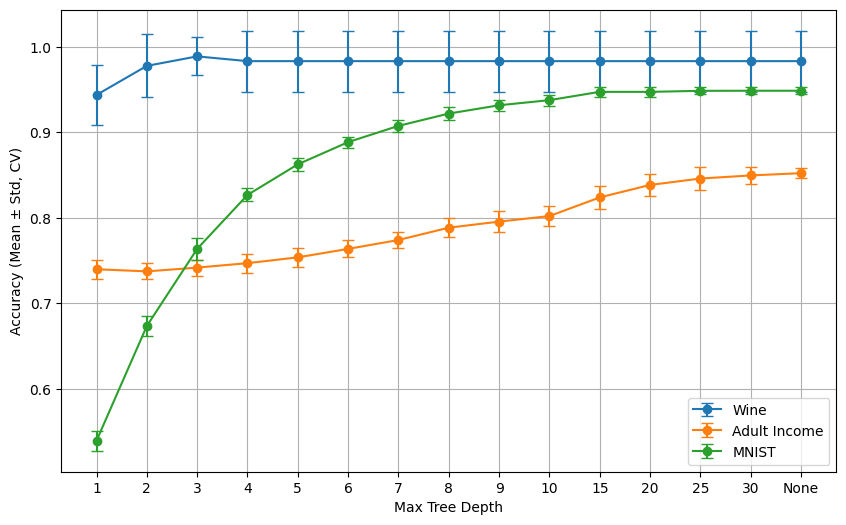
\includegraphics[width=\linewidth]{figures/accuracy_vs_depth.png}
    \caption{Accuracy vs. Max Depth}
    \label{fig:accuracy_vs_depth}
\end{figure}

For more complex datasets such as the adult income dataset, the accuracy starts at a lower point and gradually increases with deeper trees. When no maximum depth is set, the accuracy reaches its highest point. This indicates that for complex datasets, deeper trees are beneficial as they can capture more intricate patterns in the data.

The MNIST dataset, being the most complex of the three, shows a significant increase in accuracy with deeper trees. The accuracy grows rapidly as the depth increases from 1 to 10, after which improvements become minimal and the accuracy plateaus. This suggests that for highly complex datasets, deeper trees are necessary to effectively model the data, but there is a point of diminishing returns where further increases in depth yield minimal gains in performance.

\begin{figure*}[htbp]
    \centering
    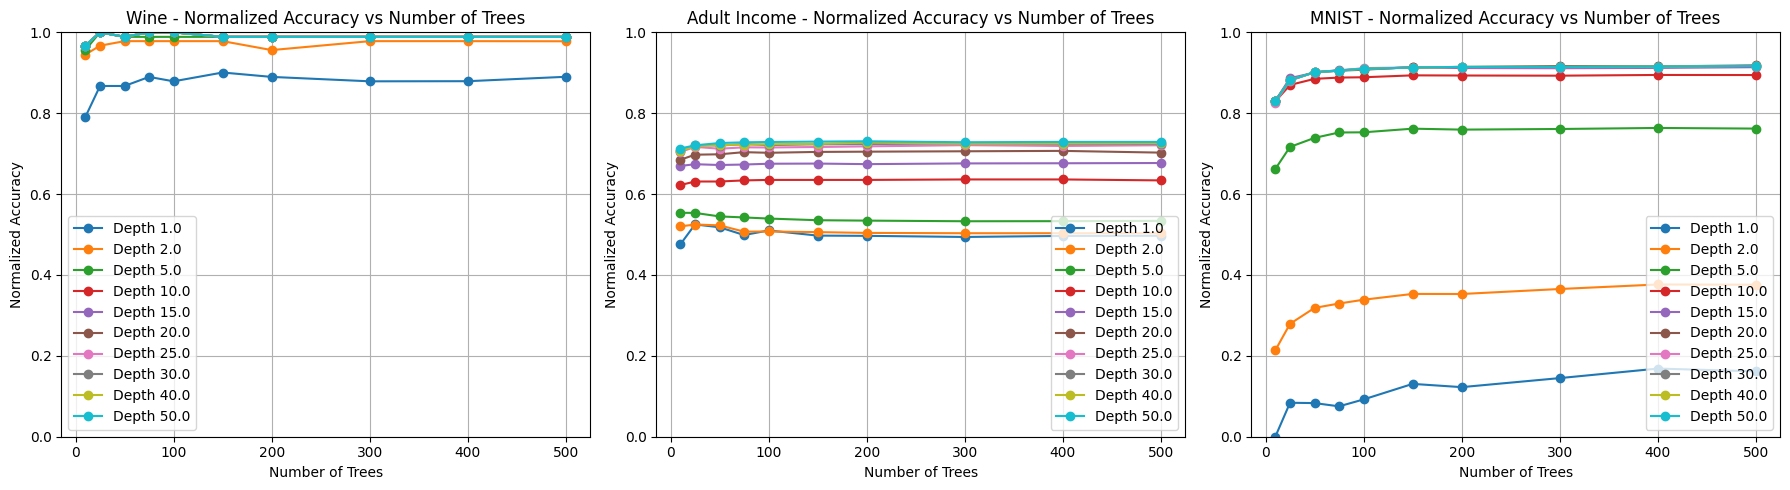
\includegraphics[width=\textwidth]{figures/line_plot_exp_2.png}
    \caption{Accuracy vs. Number of Trees (Experiment 2)}
    \label{fig:accuracy_vs_trees_exp_2}
\end{figure*}

Figure~\ref{fig:accuracy_vs_trees_exp_2} presents the accuracy results from \textit{Experiment 2}, which investigates the relationship between the number of trees and tree depth. For the wine dataset, accuracy remains relatively stable across different ensemble sizes, indicating that a small number of trees suffices for this simple dataset. Figure~\ref{fig:heatmaps_exp_2} shows heatmaps of accuracy; for the wine dataset, rows from depth 10 onward are largely identical, which emphasises the finding from \textit{Experiment 1} that deeper trees do not significantly improve performance. For this dataset, increasing the number of trees has little effect on accuracy.

For the adult income dataset, accuracy increases modestly as the number of trees grows, with most gains occurring when the ensemble size increases from 10 to 50; thereafter accuracy stabilises.

\begin{figure*}[htbp]
    \centering
    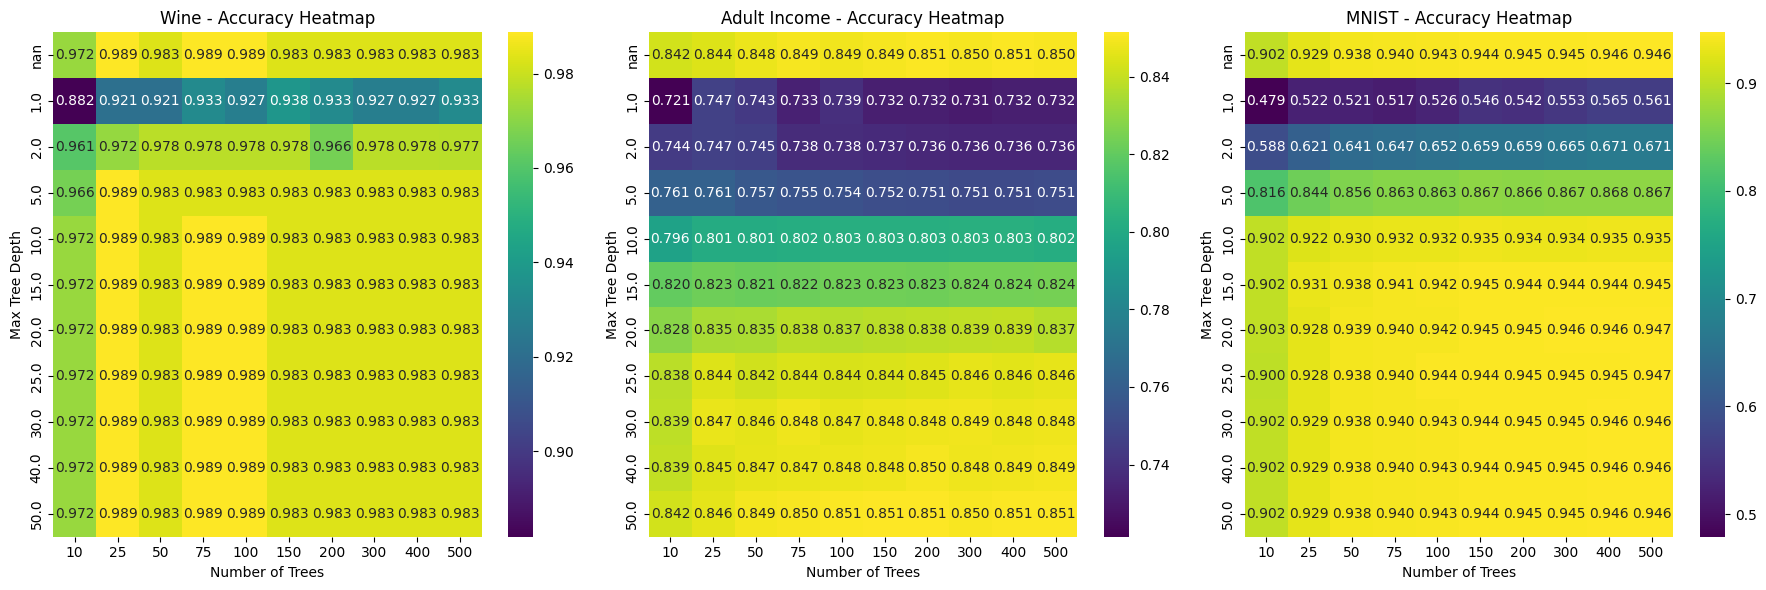
\includegraphics[width=\textwidth]{figures/heatmaps_exp_2.png}
    \caption{Heatmaps of Accuracy for Experiment 2}
    \label{fig:heatmaps_exp_2}
\end{figure*}

The MNIST dataset benefits most from additional trees in these experiments: accuracy increases substantially as the number of trees grows from 10 to about 150, after which gains are minimal and accuracy stabilises.

Overall, the results from \textit{Experiment 2} indicate that while increasing the number of trees can improve accuracy, the magnitude of improvement depends on dataset complexity. Simple datasets such as the wine dataset show little benefit from additional trees, whereas complex datasets such as MNIST show larger gains, albeit with diminishing returns as ensemble size increases.

Figure~\ref{fig:acc_vs_max_feat_exp_3_2} presents the accuracy results from \textit{Experiment 3}, which varied the number of features considered at each split. The wine and adult income datasets have 13 and 14 features, respectively; once \texttt{max\_features} reaches the dataset dimensionality the accuracy stabilises. For the wine dataset, accuracy is highest when a single feature is selected per split and decreases as more features are allowed. This observation suggests that, for simple datasets, selecting fewer features per split can reduce overfitting and increase tree diversity.

The adult income dataset exhibits relatively stable accuracy across the tested \texttt{max\_features} values. The best observed accuracy occurred when no limit was set and when 50\% of the features were used; report the numeric best value here.

\begin{figure}
    \centering
    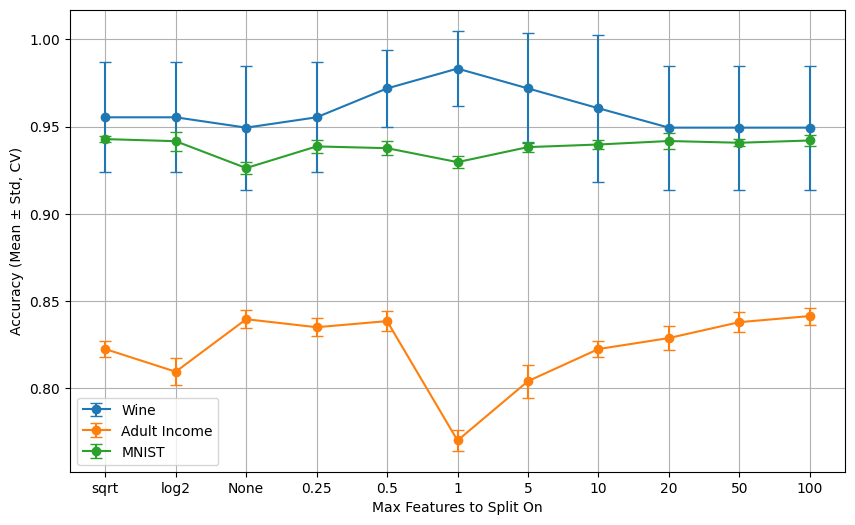
\includegraphics[width=\linewidth]{figures/acc_vs_max_feat_exp_3_2.png}
    \caption{Accuracy vs. Max Features (Experiment 3)}
    \label{fig:acc_vs_max_feat_exp_3_2}
\end{figure}

For MNIST, accuracy increases as more features are considered. The tested settings included single-feature splits, fixed counts up to 100 features, fractional settings (25\%, 50\%), and no limit. Accuracy rises rapidly from the smallest settings up to larger counts, and is highest for the larger fractions or when no limit is applied; report the numeric peak and its corresponding setting.

Figure~\ref{fig:uncertainty_diversity} presents the values of uncertainty and diversity for each dataset across the multiple folds from \textit{Experiment 4}, which evaluated a heterogeneous ensemble of decision trees with varying parameters. The wine dataset exhibits a relatively high level of uncertainty, with values for each fold ranging between 0.35 and 0.4. This suggests that the ensemble's predictions are less confident, which may be related to the dataset's simplicity and the limited number of features available for splitting. Diversity values are also high (0.2 to 0.4), indicating that individual trees make varied predictions. Such diversity can reduce correlation among trees and improve overall ensemble performance.

The adult income dataset demonstrates high uncertainty (0.29 to 0.32) and low diversity (0.12 to 0.15). This means the ensemble's predictions are not very confident, and the individual trees tend to make similar predictions. Low diversity may limit the effectiveness of the ensemble, as correlated trees do not provide the error-correcting benefits associated with more diverse models.

For the MNIST dataset, both uncertainty and diversity values are low (below 0.1), indicating that the ensemble makes confident and consistent predictions. This is expected given the dataset's complexity and the large number of features available for splitting. The low diversity suggests that individual trees produce similar outputs, likely due to the high dimensionality of the data, which can lead to correlated tree behavior.

In summary, the results show that ensemble diversity and uncertainty are strongly influenced by dataset complexity and feature dimensionality. High diversity in ensemble methods is generally beneficial, but must be balanced with prediction confidence for optimal performance.
\begin{figure*}[htbp]
    \centering
    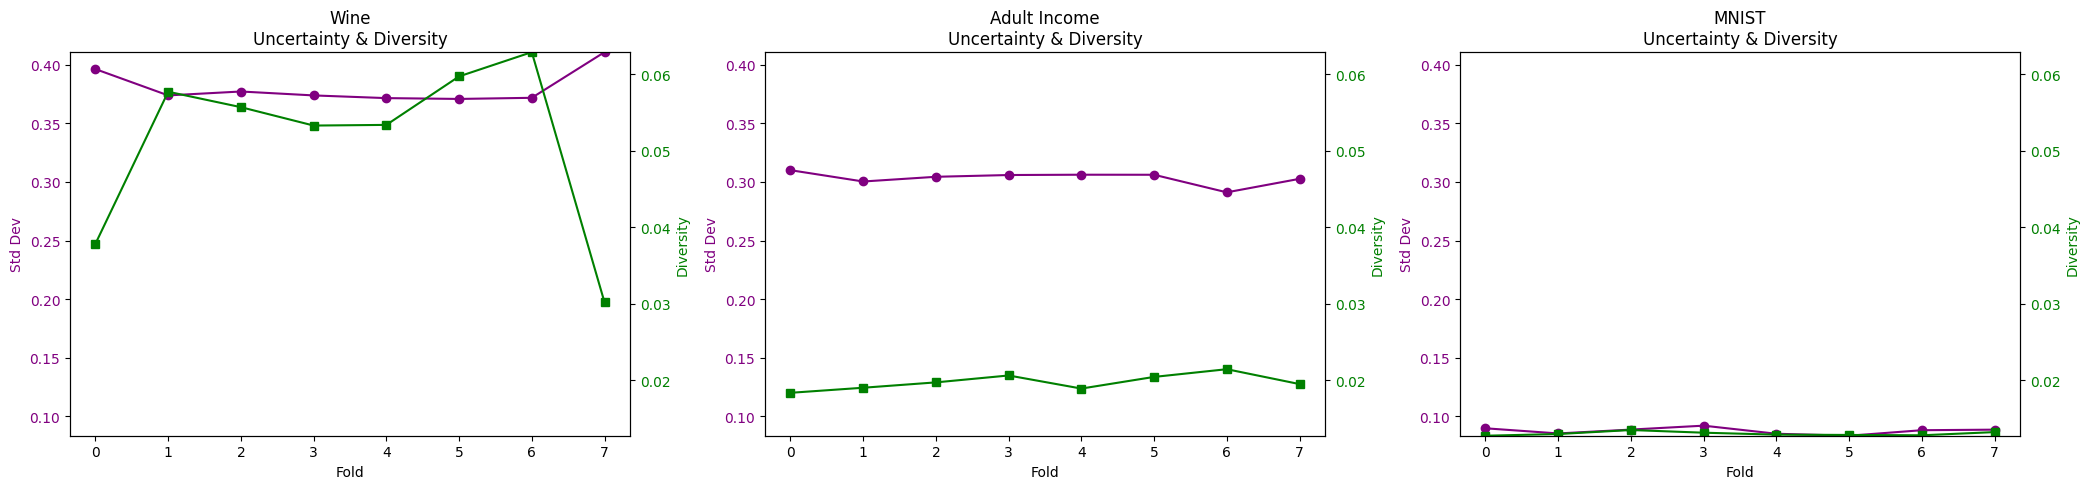
\includegraphics[width=\textwidth]{figures/uncertainty_diversity.png}
    \caption{Scatterplots of Uncertainty and Diversity for Experiment 4}
    \label{fig:uncertainty_diversity}
\end{figure*}

\begin{figure*}[htbp]
    \centering
    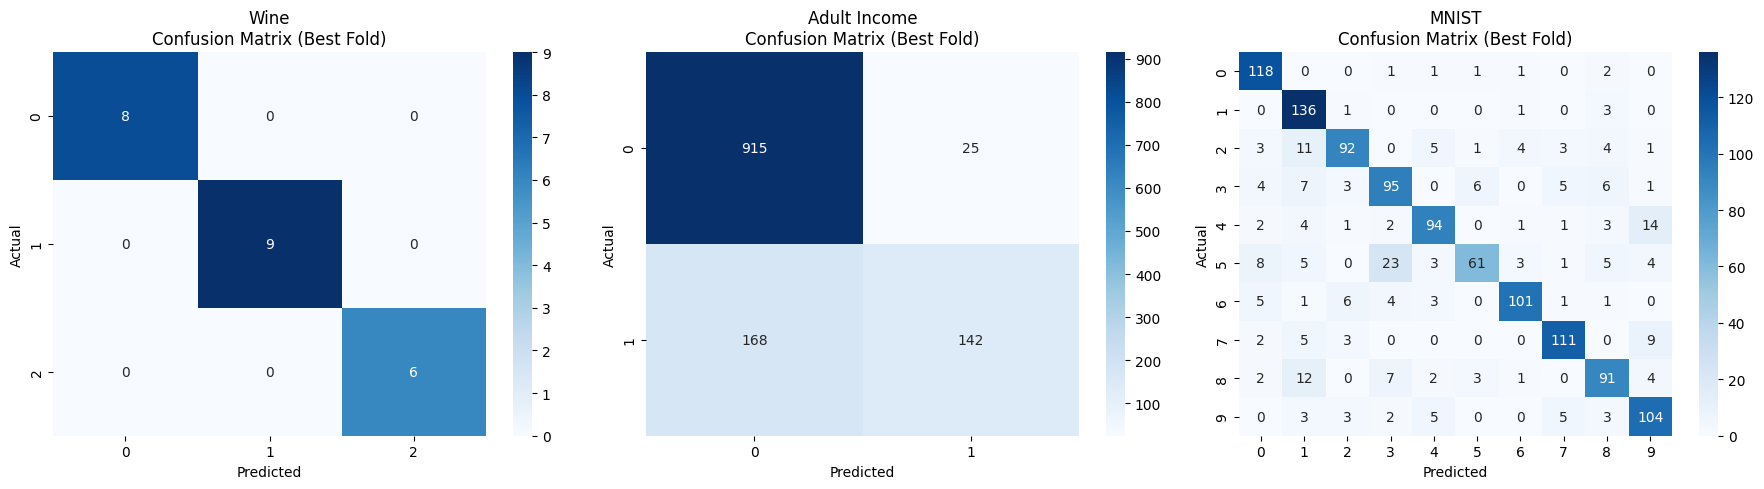
\includegraphics[width=\textwidth]{figures/confusion_exp_4.png}
    \caption{Confusion Matrices for Experiment 4}
    \label{fig:confusion_matrix_best_model}
\end{figure*}

\section{Conclusion}

This assignment provided a comprehensive investigation into the impact of key parameters on the performance of random forests across datasets of varying complexity. Through systematic experimentation, the effects of tree depth, number of features considered at each split and the relationship of the number of trees and tree depth were explored, along with the performance of heterogeneous ensembles with diverse tree configurations.

The results demonstrated that datasets of different complexities require different parameter settings. For simple datasets such as the wine dataset, shallow trees and fewer features per split were sufficient to achieve high accuracy, while more complex datasets benefited from deeper trees and a greater number of features. Increasing the number of trees generally improved performance, but with diminishing returns beyond a certain point. The analysis of uncertainty and diversity revealed that ensemble confidence and tree heterogeneity are influenced by both data complexity and feature dimensionality.

Overall, the findings highlight the importance of careful parameter tuning and the value of ensemble diversity in achieving robust and accurate models.

\bibliographystyle{IEEEtran}
\bibliography{refs}
\end{document}
